

\documentclass[conference]{IEEEtran}


\usepackage{amsfonts}
\usepackage{amssymb}
\usepackage{amsmath}
\interdisplaylinepenalty=2500
\usepackage{graphicx}
\usepackage{subfigure}
\usepackage{mathrsfs}
\usepackage{cite}
\usepackage{algorithm}
\usepackage{algorithmic}
\usepackage{flushend}
\usepackage{tikz} % ��������

% correct bad hyphenation here
\hyphenation{op-tical net-works semi-conduc-tor}


\begin{document}
%
% paper title
% Titles are generally capitalized except for words such as a, an, and, as,
% at, but, by, for, in, nor, of, on, or, the, to and up, which are usually
% not capitalized unless they are the first or last word of the title.
% Linebreaks \\ can be used within to get better formatting as desired.
% Do not put math or special symbols in the title.
\title{$Q$-Learning Based Power Control Algorithm\\ for D2D Communication}


% author names and affiliations
% use a multiple column layout for up to three different
% affiliations
\author{
%\IEEEauthorblockN{Shiwen Nie}
%\IEEEauthorblockA{Beijing University of Posts and \\Telecommunications \\
% Haidian District,Beijing30332--0250\\
%Email: http://www.michaelshell.org/contact.html}
%\and
\IEEEauthorblockN{Shiwen Nie, Zhiqiang Fan, Ming Zhao, Xinyu Gu, Lin Zhang}
%\IEEEauthorblockA{Twentieth Century Fox\\
%Springfield, USA\\
%Email: homer@thesimpsons.com}
\IEEEauthorblockA{Key Lab of Universal Wireless Communication\\
Beijing University of Posts and Telecommunications,Beijing,China 100876\\
Email: 2014110444@bupt.edu.cn}
%\and
%\IEEEauthorblockN{Xinyu Gu}
%\IEEEauthorblockA{Starfleet Academy\\
%San Francisco, California 96678--2391\\
%Telephone: (800) 555--1212\\
%Fax: (888) 555--1212}
}

% conference papers do not typically use \thanks and this command
% is locked out in conference mode. If really needed, such as for
% the acknowledgment of grants, issue a \IEEEoverridecommandlockouts
% after \documentclass

% for over three affiliations, or if they all won't fit within the width
% of the page, use this alternative format:
%
%\author{\IEEEauthorblockN{Michael Shell\IEEEauthorrefmark{1},
%Homer Simpson\IEEEauthorrefmark{2},
%James Kirk\IEEEauthorrefmark{3},
%Montgomery Scott\IEEEauthorrefmark{3} and
%Eldon Tyrell\IEEEauthorrefmark{4}}
%\IEEEauthorblockA{\IEEEauthorrefmark{1}School of Electrical and Computer Engineering\\
%Georgia Institute of Technology,
%Atlanta, Georgia 30332--0250\\ Email: see http://www.michaelshell.org/contact.html}
%\IEEEauthorblockA{\IEEEauthorrefmark{2}Twentieth Century Fox, Springfield, USA\\
%Email: homer@thesimpsons.com}
%\IEEEauthorblockA{\IEEEauthorrefmark{3}Starfleet Academy, San Francisco, California 96678-2391\\
%Telephone: (800) 555--1212, Fax: (888) 555--1212}
%\IEEEauthorblockA{\IEEEauthorrefmark{4}Tyrell Inc., 123 Replicant Street, Los Angeles, California 90210--4321}}


% make the title area
\maketitle

% As a general rule, do not put math, special symbols or citations
% in the abstract
\begin{abstract}
%Device-to-Device (D2D) has become a promising approach to improve the spectrum efficiency of cellular network, and power control turns out to be an important method for interference management when D2D users share the same frequency band with cellular users.
 In this paper, power control algorithm based on reinforcement learning (RL) in underlay D2D communication is studied. The approach we use regards D2D communication as a multi-agents system, and power control is achieved by maximizing system capacity while maintaining the requirement of quality of service(QoS) from cellular users. We propose two RL based power control methods for D2D users, i.e., team-$Q$ learning and distributed-$Q$ learning. The former is a centralized method in which only one $Q$-value table needs to be maintained, while the latter enables D2D users to learn independently and reduces the complexity of $Q$-value table. Simulation results show the difference of the two $Q$-learning algorithm in terms of convergence and reward function. In addition, it is shown that through our distributed-$Q$ learning, D2D users not only are able to learn their power in a self-organized way, but also achieve better system performance than that using traditional method in LTE(Long Term Evolution).
\end{abstract}

% no keywords
\begin{IEEEkeywords}
 Reinforcement learning, multi-agent system, $Q$-learning, power control, D2D communication
\end{IEEEkeywords}



% For peer review papers, you can put extra information on the cover
% page as needed:
% \ifCLASSOPTIONpeerreview
% \begin{center} \bfseries EDICS Category: 3-BBND \end{center}
% \fi
%
% For peerreview papers, this IEEEtran command inserts a page break and
% creates the second title. It will be ignored for other modes.
\IEEEpeerreviewmaketitle



\section{Introduction}
%With the emerging of a myriad of smart handheld devices and the drastic growth of
%bandwidth-hungry applications such as video streaming and multimedia file sharing, mobile users'
%demands for spectrum in current cellular system are undergoing an unprecedented rise
%\cite{tehrani2014device}.

%higher-performance traffic with fewer energy cost.
%(Reducing energy consumption in wireless communications has attracted increasing attention recently.)
The popularity of mobile Internet promotes a myriad of smart handheld devices as well as many energy-hungry and bandwidth-hungry applications, such as video streaming and multimedia file sharing, mobile P2P, 3D services\cite{feng2013survey,tehrani2014device}. On the energy side, transmissions for the large amount of mobile data have caused great energy consumption, which occupies a huge proportion of total consumed energy for the communication networks. According to most update research reports, the energy consumption of telecommunication devices accounts for 25\% of the energy consumption in the information and communications technologies. Therefore, energy-efficient techniques need to be integrated into the next generation cellular network to reduce the energy consumption, and energy saving has been considered as a critical technology in 5G technologies. Besides, the battery life of the mobile devices has become a big limitation for the energy-hungry applications. On the bandwidth side, to meet the booming demand for spectrum and improve the spectrum efficiency of cellular system, new technologies such as Device-to-Device (D2D) communication has been proposed \cite{kaufman2008cellular,doppler2009device,peng2009interference}. D2D communication technology is not only able to support smaller communication latency and higher spectrum efficiency\cite{belleschi2011performance}, but also able to potentially improve throughput, energy consumption and fairness, which makes it a promising technology for future 5G network.

Energy efficiency (EE) optimization has always been an important issue in wireless communications and gains more attention. For example, \cite{shams2014energy,shams2014q,zhang2014qos,chen2013improving} formulate the EE issue as a fractional programming problem. Specifically, \cite{shams2014energy} studied the resource allocation in multi-cell OFDMA system, \cite{shams2014q,zhang2014qos,chen2013improving} studied the joint resource and power allocation problems appear in OFDMA system. It has been noticed that EE optimization problem is of non-convex and fractional nature[14], and plenty of the studies on this issue \cite{shams2014energy,shams2014q,zhang2014qos,chen2013improving} use a centralized approach.

Recently, energy-efficient technique has also been of great interest in D2D communications. Compared to the centralized approach proposed in \cite{shams2014energy,shams2014q,zhang2014qos,chen2013improving}, D2D communication prefers a distributive way. For example, \cite{wu2014energy,zhou2015game,zhou2014distributed,wang2015energy} studied the distributed energy-efficient resource allocation problem with Quality of Service (QoS) requirements in mobile D2D communications. In \cite{akkarajitsakul2012mode}, the mode selection problem with transmission rate constraints was considered in D2D communications under LTE-advanced networks. \cite{wen2013energy,wu2015optimal} studied the energy-efficient power control schemes in D2D communications. [14] developed power control algorithms for EE in both centralized and distributed way, where game theory is used to study the equilibria of the network in the distributed case.

Actually, game theory has become a powerful tool to study distributed power control for energy efficient in wireless networks. For example, \cite{saraydar2002efficient} formulated the distributed power control as a non-cooperative game and showed that its Nash equilibrium is inefficient, but it found that pricing of transmit powers can improve efficiency. Pricing method can also be found in \cite{jang2014energy} where the EE uplink power control was studied for multiuser SIMO system. \cite{miao2011distributed} use game theory to develop an energy-efficient power optimization scheme for multi-cell interference-limited wireless communications and studies the existence of equilibrium. However, game theory used in \cite{saraydar2002efficient,jang2014energy,miao2011distributed} requires the assumption that transmitter is of continuous power value, which is actually discrete in practical system. Studies with the assumption of discrete transmission power can be found in [18,19]. In [18], a no-cooperative power control algorithm with repeated games in Ad hoc networks was developed, where the opponents�� historical joint behavior is required and it was showed that the proposed algorithm eventually converged to pure Nash Equilibrium (NE). [19] uses stochastic iterative procedures to perform the strategy evaluation of game and studied its convergence and stability theoretically.

Recent trends of using game theory in wireless communication community has focused on the combination with machine learning approaches, especially reinforcement learning (RL) method. $Q$-learning is a basic RL algorithm and is supposed to be an effective way for energy efficient power control. For example, \cite{shams2014energy,shams2014q} used $Q$-learning in multiple-relay cooperative networks to improve  Energy Efficiency. \cite{zhang2014qos,chen2013improving} applied $Q$-learning combining with Stackelberg game framework for power control in femto-cell networks. \cite{wang2013distributed} proposed an $Q$-learning  based asynchronous dynamic power allocation among femto-cells to mitigate the interference in the cellular network. \cite{hybrid2015maghsudi} studied resource allocation and power control problem in D2D communication and used $Q$-learning better-reply dynamics to achieve equilibrium.
%To avoid the complexity incurred by a pricing mechanism,

In this paper, we model the D2D underlaying cellular network as a multi-agent system and develop two approaches based on $Q$-learning for energy efficient power control. The first approach is to minimize each user's transmission power to reduce power consumption and protect the quality of service (Qos) of D2D users at the same time. However, we find that energy efficiency of each user is not improved, although energy consumption is reduced. Thus, in our second $Q$-learning based approach, each user tries to maximize their own energy efficiency, which is defined as the user's reward function.

%%% ���ɾ�ˣ�������ǰ���Ҹ����ʵ�λ��
%In multi-agent system, since the reward function which includes other agents' action or reward information, every agent reward will be influenced by other agents, needs to be implemented in a both of two approaches can be implemented in distributed way, thus agents learn by themselves and avoid too much overhead.

The main contributions of this paper are two-folds:
\begin{itemize}
  \item We propose two algorithms based on $Q$-learning for power control in
      underlaying D2D communication to enhance the system capacity while maintaining the QoS of the cellular users.
  \item We make improvement of the reward function to make D2D users learn in a distributive manner so that both computational complexity and the amount of required feedback information with guaranteeing system performance can be reduced. In addition, the new reward function is compared to that used in \cite{saad2014cooperative}.
\end{itemize}
The rest of this paper is organized as follows. Section II describes the model of the system and formulates the problem. Section III introduces two methods of $Q$-learning for power control, including team-$Q$ and distributed-$Q$ algorithm. Section IV presents simulation results and analysis. Section V concludes this paper.



% An example of a floating figure using the graphicx package.
% Note that \label must occur AFTER (or within) \caption.
% For figures, \caption should occur after the \includegraphics.
% Note that IEEEtran v1.7 and later has special internal code that
% is designed to preserve the operation of \label within \caption
% even when the captionsoff option is in effect. However, because
% of issues like this, it may be the safest practice to put all your
% \label just after \caption rather than within \caption{}.
%
% Reminder: the "draftcls" or "draftclsnofoot", not "draft", class
% option should be used if it is desired that the figures are to be
% displayed while in draft mode.
%
%\begin{figure}[!t]
%\centering
%\includegraphics[width=2.5in]{myfigure}
% where an .eps filename suffix will be assumed under latex,
% and a .pdf suffix will be assumed for pdflatex; or what has been declared
% via \DeclareGraphicsExtensions.
%\caption{Simulation results for the network.}
%\label{fig_sim}
%\end{figure}

% Note that the IEEE typically puts floats only at the top, even when this
% results in a large percentage of a column being occupied by floats.


% An example of a double column floating figure using two subfigures.
% (The subfig.sty package must be loaded for this to work.)
% The subfigure \label commands are set within each subfloat command,
% and the \label for the overall figure must come after \caption.
% \hfil is used as a separator to get equal spacing.
% Watch out that the combined width of all the subfigures on a
% line do not exceed the text width or a line break will occur.
%
%\begin{figure*}[!t]
%\centering
%\subfloat[Case I]{\includegraphics[width=2.5in]{box}%
%\label{fig_first_case}}
%\hfil
%\subfloat[Case II]{\includegraphics[width=2.5in]{box}%
%\label{fig_second_case}}
%\caption{Simulation results for the network.}
%\label{fig_sim}
%\end{figure*}
%
% Note that often IEEE papers with subfigures do not employ subfigure
% captions (using the optional argument to \subfloat[]), but instead will
% reference/describe all of them (a), (b), etc., within the main caption.
% Be aware that for subfig.sty to generate the (a), (b), etc., subfigure
% labels, the optional argument to \subfloat must be present. If a
% subcaption is not desired, just leave its contents blank,
% e.g., \subfloat[].


% An example of a floating table. Note that, for IEEE style tables, the
% \caption command should come BEFORE the table and, given that table
% captions serve much like titles, are usually capitalized except for words
% such as a, an, and, as, at, but, by, for, in, nor, of, on, or, the, to
% and up, which are usually not capitalized unless they are the first or
% last word of the caption. Table text will default to \footnotesize as
% the IEEE normally uses this smaller font for tables.
% The \label must come after \caption as always.
%
%\begin{table}[!t]
%% increase table row spacing, adjust to taste
%\renewcommand{\arraystretch}{1.3}
% if using array.sty, it might be a good idea to tweak the value of
% \extrarowheight as needed to properly center the text within the cells
%\caption{An Example of a Table}
%\label{table_example}
%\centering
%% Some packages, such as MDW tools, offer better commands for making tables
%% than the plain LaTeX2e tabular which is used here.
%\begin{tabular}{|c||c|}
%\hline
%One & Two\\
%\hline
%Three & Four\\
%\hline
%\end{tabular}
%\end{table}


% Note that the IEEE does not put floats in the very first column
% - or typically anywhere on the first page for that matter. Also,
% in-text middle ("here") positioning is typically not used, but it
% is allowed and encouraged for Computer Society conferences (but
% not Computer Society journals). Most IEEE journals/conferences use
% top floats exclusively.
% Note that, LaTeX2e, unlike IEEE journals/conferences, places
% footnotes above bottom floats. This can be corrected via the
% \fnbelowfloat command of the stfloats package.


\section{SYSTEM MODEL AND PROBLEM FORMULATION}

In this section, we first describe the system model of underlaying D2D communication, then the problem formulation is given.

\subsection{System Model}

The system model is given by Fig. 1. We consider the uplink (UL) transmission in a single cell which consists of $M$ cellular users sharing there resource blocks (RBs) with $N$ D2D users. The cellular users and D2D users are denoted by $\mathcal{M} = \{1, \ldots, M \}$ and $\mathcal{N} = \{ 1,\ldots, N \}$ respectively. The available RBs for cellular users are denoted by $K$. It is assumed that the location of D2D pairs follows a uniform distribution within the coverage of base station (BS). It is further assumed that each RB is occupied by only one cellular user and can be shared with multiple D2D pairs. Thus, there are two kinds of interference, i.e., one is from D2D transmitter to BS, the other is from cellular user and other D2D pairs who share the same RB to D2D receiver.

\begin{figure}[!t]
\centering
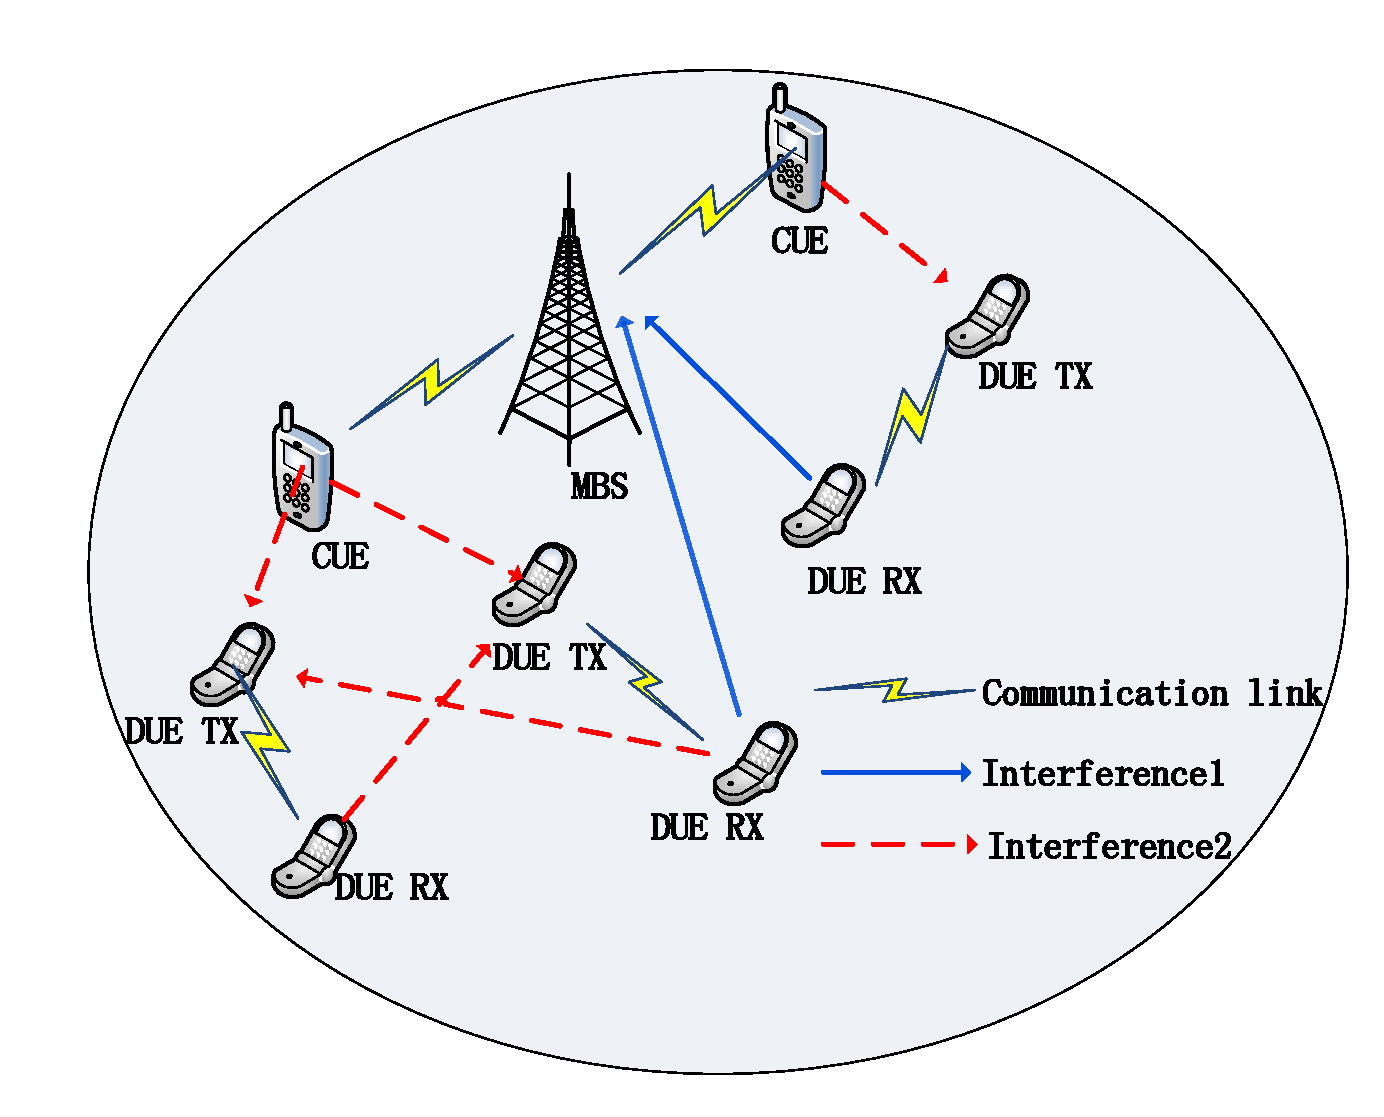
\includegraphics[width=2.5in]{pics/scenario.pdf}
\caption{D2D communication underlaid with cellular networks}
\label{fig_1}
\end{figure}

The main factor influencing link quality is the signal to interference-plus-noise ratio (SINR). In our model, the SINR for $i$th D2D user transmitting on the $k$th RB is given by

\begin{equation}
\label{eqa_1}
\gamma_k^{d_i} = \frac{p_k^{{d_i}} \cdot g_{d_i,k}^{ii}}{{\sigma ^2} + p_k^m \cdot g_{k}^{mi} +
\sum\limits_{j \in {\Re_k}}^{j \ne i} {p_k^{{d_j}} \cdot g_{d_j,k}^{ji}} } ,~~i=1,2,\ldots,N
\end{equation}

where $p_k^{d_i}$ and $p_k^m$ denote the $i$th D2D user and cellular user uplink transmission power on $k$th RB respectively, $p_{\max}$ is the upper bound of each D2D user's transmit power with $p_k^{d_i}\leq p_{\max}, \forall i\in\mathcal{N} $. $g_{d_i,k}^{ii}$, $g_{d_j,k}^{ji}$ and $g_{k}^{mi}$ represent, respectively, channel gain in $i$th D2D link, channel gain from D2D transmitter $j$ to receiver $i$ and channel gain from cellular transmitter $m$ to receiver $i$. $\Re_k$ is a D2D pairs set sharing $k$th RB. Likewise, the SINR of a cellular user $m\in\mathcal{M}$ on the $k$th RB is

\begin{equation}
\label{eqa_2}
\gamma_k^m = \frac{p_k^m \cdot {g^0}_{m,k}}{\sigma ^2 + \sum\limits_{j\in\Re_k} {p_k^{d_j} \cdot g_{j,k}^{j0}} }
\end{equation}

Where $g_{m,k}^0$ and $g_{j,k}^{j0}$ indicate the channel gain on the $k$th RB from BS to cellular user $m$ and $j$th D2D transmitter respectively.

\subsection{Formulation of Problem}

We focus on the system performance including D2D pair capacity and system capacity. Besides, it is assumed that the resource allocation and transmit power of cellular users are given and fixed. Then, the power control of D2D users can be achieved by solving problem (3):

\begin{equation}
\label{eqa_3}
\begin{array}{rl}
  \underset{\mathbf{p_k}}{\max} & \sum\limits_{k = 1}^K { \{ {{\log }_2}(1 + \gamma_k^m) + \sum\limits_{i \in {\Re _k}}^{} {{{\log }_2}(1 + \gamma_k^{d_i})} \} } \\

  ~&~\\
  s.t. &  \gamma_k^m \ge {\tau _0}\\
  ~ &  0 \leq p_k^{{d_i}} \le {p_{\max }}, \forall i,k\\
%  ~ &    \sum\limits_{k = 1}^K  \sum\limits_{i \in {\Re _k}}i \leq N
\end{array}
\end{equation}


%Ϊ�˰ѹ�ʽ���ڵ�ǰҳ

\begin{figure*}[!ht]
\begin{equation*}
Q_{t+1}(s_t,a_t) =
\begin{cases}
Q_t(s_t,a_t) + \alpha\big[r_{t+1} + \gamma~ \underset{{a^\prime}}{\max}~ Q_t(s_{t+1},a_{t+1}) - Q_t(s_t,a_t)\big] & \text{ if } s=s_t \text{ and }
a=a_t,\\
Q_t(s_t,a_t) & \text{ otherwise,}
\end{cases}
\eqno{(9)}
\end{equation*}
\hrulefill
\vspace*{4pt}
\end{figure*}



where $\mathbf{p_k}=(p_k^{{d_1}},\cdots,p_k^{{d_i}},\cdots,p_k^{{d_N}})$. The object function to be maximized is the network capacity and the constraints including QoS requirement of cellular users, maximum power of transmitters. It is obvious that, on the one hand, as D2D user's transmitter power increases, D2D throughout will increase while cellular users will suffer more interference. On the other hand, the constraints to ensure the QoS of cellular users will limit D2D users' power. To figure out the optimal $p_k^{{d_i}}$, the RL based power control algorithm will be introduced.




\section{REINFORCEMENT LEARNING BASED POWER CONTROL ALGORITHM}

In this section, we first introduce Q-learning algorithm in single-agent case to illustrate learning process. Subsequently, two Q-learning based power control algorithms are presented. Furthermore, a new reward function is adopted to make agents learn independently, where only local information is used.


\subsection{Single-agent $Q$-Learning Algorithm}

$Q$-learning is a form of model-free reinforcement learning , which learns optimal policy by interacting with environment. Moreover, there is no need for the prior knowledge about state transition probability function and reward function.

$Q$-learning is represented by a tuple $<(S, A, T, R(s,a))>$, where $S$ is the finite set of environment states, $A$ is the finite set of agent actions, $T : S \times A \times S \mapsto [0, 1]$ is the state transition probability function, and $R: S \times A \times S \mapsto R$ is the reward function. In the interaction process between an agent $i$ and environment, agent $i$ senses current state $s_t^i\in S$ and selects an action $a_t^i \in A$ according to policy $\pi$, which is a function define as $\pi:S \mapsto A$. As a result, the environment makes a transition to new state $s^\prime\in S$ and a reward $r_t^i$ is fed back to agent $i$. This process will be repeated until optimal policy $\pi$ is obtained. Under a policy $\pi$, the value of a state is

\begin{equation}
\label{eqa_4}
V^\pi(s) = E_\pi \big\{ r_t|s_t=s \big\} = E_\pi \Big\{ \sum_{k=1}^\infty \gamma^k r_{t+k+1}|s_t=s
\Big\}
\end{equation}

where $0\leq \gamma\leq 1$ is a discount factor and $V^\pi(s)$ represents the expected discounted reward. Through learning repeatedly, an optimal $a^*\in A$ can be obtained by maximizing a cumulative measurement of the rewards over time. According to Bellman optimality criterion\cite{watkins1992q}, there is at least one optimal strategy $\pi^*$ in a single environment setting such that:

\begin{equation}
\label{eqa_5}
V^*(s) = V^{\pi^*}(s) = \max_a \Big\{ R(s,a) + \gamma\sum_{s^\prime \in S} P_{s,s^\prime} (a) V^*(s)
\Big\}
\end{equation}

where $R(s,a)$ is the mathematical expectation of $r(s,a)$, and $P_{s,s^\prime}$ is transition
probability  from state $s$ to state $s^\prime$.

$Q$-values (or action value) is the expected return of taking action $a$ in state s under policy $\pi$:

\begin{equation}
\label{eqa_6}
Q^\pi(s,a) = R(s,a) + \gamma\sum_{s^\prime\in S} P_{s,s^\prime}(a) Q(s^\prime,a)
\end{equation}

The optimal policy $Q^*(s,a)$ is defined as

\begin{equation}
\label{eqa_7}
Q^*(s,a) \equiv Q^{\pi^*}(s,a), \forall s,a
\end{equation}

Obviously, we obtain

\begin{equation}
\label{eqa_8}
V^*(s) = \max_a  Q^*(s,a)
\end{equation}
The $Q$-learning algorithm adjusts $Q$-value according to the update rule as described in formula (9), where $\alpha_k \in (0, 1]$ is learning rate.


%\begin{equation}
%\label{eqa_9}
%Q_{t+1}(s_t,a_t) =
%\begin{cases}
%Q_t(s_t,a_t) + \alpha[r_{t+1} + \gamma \max_{a^\prime} Q_t(s_{t+1},a_{t+1}) - Q_t(s_t,a_t)] & \text{ if } s=s_t \text{ and }
%a=a_t,\\
%Q_t(s_t,a_t) & \text{ otherwise,}
%\end{cases}
%\end{equation}


In our system, D2D transmitter in each D2D pair is treated as an agent. Since the whole network includes many agents, it can be regarded as a multi-agents system where the optimal policy of an agent depends not only on the environment but also on the policies of the other agents \cite{wiering2012reinforcement}. Thus the aforementioned $Q$-learning algorithm needs to be extended from single-agent to multi-agents. In next subsections, multi-agents $Q$-learning algorithms such as team-$Q$ \cite{littman2001value} and distributed-$Q$ \cite{lauer2000algorithm} will be introduced for power control issue arisen in problem (3).


\subsection{Multi-agent Reinforcement Learning}
In this section, we give a rudimentary introduction to the theory of multi-agent reinforcement
learning(MARL).
\begin{figure}[!h]
\centering
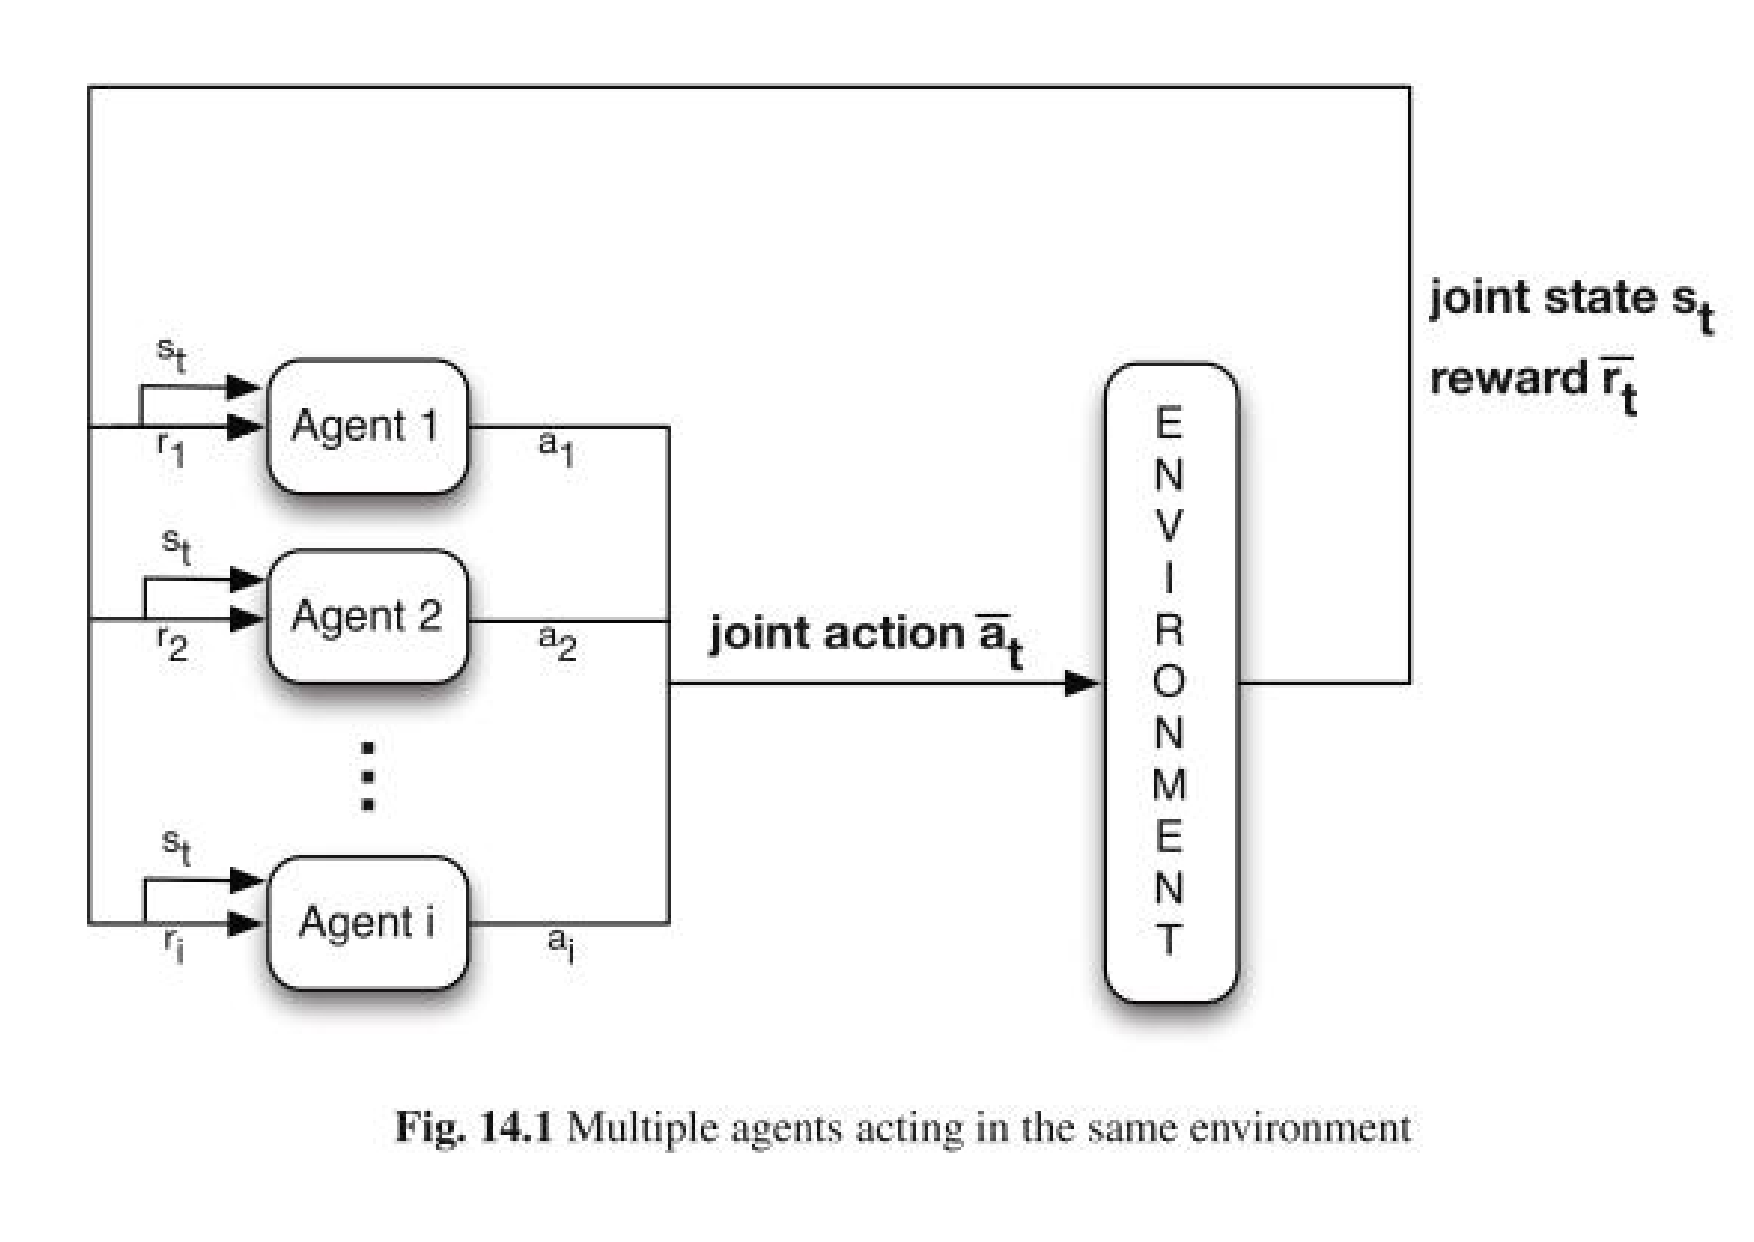
\includegraphics[width=3.3in]{pics/a1.pdf}
\caption{Heterogeneous Network with CRE technology}
\label{fig_1}
\end{figure}
Traditional reinforcement learning is developed for Markov Decision Processes (MDPs). It allows single
agent learn through trial-and-error interaction with its environment and guarantees convergence to the
optimal policy. $Q$-learning is one common reinforcement learning algorithm and learns with model-free.

In this paper, we want to extend reinforcement learning from single agent to multi-agent. In
multi-agent system, the optimal policy of an agent depends not only on the environment, but on the
policies of the other agents as well \cite{wiering2012reinforcement}. Fig.3 shows the model of standard
MARL. In such model, reward is depended on joint action and states and MDP model might be failure. The
generalization of the MDP to the multi-agent case is the stochastic game
\cite{busoniu2008comprehensive}.

Definition:  A stochastic games (SG) is define is a tuple $(N,S,A_{1,2,\ldots,n},T,R_{1,2,\ldots,n})$
\begin{itemize}
   \item  $N$ is the number of agent
   \item  $S$ is a finite set of states of the environment;
   \item  $A_k$ is the discrete sets of actions available to the agent $k$;
   \item  $R_k :S\times A_1 \times \ldots \times A_n \mapsto R, i=1,2,\ldots,n$ are the rewards of
       agent $k$.
   \item  $T$ is the transition probability function.
 \end{itemize}

Stochastic games were more recently proposed as the standard framework for multi-agent reinforcement
learning \cite{wiering2012reinforcement}. Based on the type of task, MARL algorithms are classified
into fully cooperative, fully competitive, and mixed games.In multi-agent system, if stochastic games
focus on dealing with multi-agent interactions with only one state, it is stateless game or repeated
game. Stochastic games can be seen as an extension of repeated games to multiple state case and MDPs
to the multi-agent case.

There is a real need for MARL. However, it still poses challenges. Besides challenges inherited from
single-agent RL, including the curse of dimensionality and the exploration-exploitation tradeoff,
several new challenges arise in MARL: the difficulty of specifying a learning goal, the non-stationary
of the learning problem, and the need for coordination \cite{busoniu2008comprehensive}.

In our considered system of N D2D pairs, each D2D pair has to learn the strategies in terms of power
control with the concern of maximizing the system capacity while maintaining the QoS requirement of
cellar users. Based on the type of task, MARL algorithms are classified into fully cooperative, fully
competitive, and mixed games.In multi-agent system, if stochastic games focus on dealing with multi-agent
interactions with only one state, it is stateless game or repeated game. Stochastic games can be seen
as an extension of repeated games to multiple state case and MDPs to the multi-agent case.


\subsection{$Q$ Learning Based Power Control for minimize transmission power}

In order to reduce energy consumption, we develop a Q learning based power control to minimize total transmission power. Notice that problem (3) can decompose into $K$ parallel power control task, thus solving (3) with $Q$-learning algorithm naturally decomposes into $K$-parallel learning task running on each RB.

Consider learning on one RB, denoted by RB $k$. Let $\Re_k=\{1,2,,\ldots,n\}$ represent the set of users sharing RB $k$. To make this method can be implement in distributed way, the problem of minimizing total transmission power change into that each D2D user $i$ in $R_k$ tries to minimize its own transmission power while satisfy the Qos of D2D user over given discrete sets of available power levels. Therefore the problem can be formulated as follows.

\begin{equation}
\label{eqa_3}
\begin{array}{rl}
  \underset{\mathbf{p_k}}{\min} & p^k \\

  ~&~\\
  s.t. &  \gamma_k^m \ge {\tau _0}\\
  ~ &  0 \leq p_k^{{d_i}} \le {p_{\max }}, \forall i,k\\
%  ~ &    \sum\limits_{k = 1}^K  \sum\limits_{i \in {\Re _k}}i \leq N
\end{array}
\end{equation}


In $Q$ learning, the agents, states, actions and reward function are defined as follows:

\newtheorem{definition}{Definition}
\textbf{Agent:}
The agents are D2D transmitters. A D2D transmitter is denoted by D2D $i$, $1\leq i \leq n$



\begin{figure*}[!t]
\begin{equation}\tag{14}
Q_{t+1}(s_t,a_t) =
\begin{cases}
\max\big\{~Q_t(s_t,a_t) , ~ r_{t+1} + \gamma~ \underset{a^\prime}{\max}~ Q_t(s_{t+1},a_{t+1}) \big\} & \text{ if } s=s_t \text{ and }
a=a_t,\\
Q_t(s_t,a_t) & \text{ otherwise,}
\end{cases}
\end{equation}
\hrulefill
\vspace*{4pt}
\end{figure*}




\textbf{State:}
The state of D2D user $i$ on RB $k$ at time $t$ is defined as:
$$\mathcal{S}_t^{i,k} = \{I_t^{k}\}$$
where $I_t^{k}\in\{0, 1\}$ indicates the level of interference measured by the cellular user on RB $k$ at time $t$, which is defined by

\setcounter{equation}{9}
\begin{equation}
\setlength{\nulldelimiterspace}{0pt}
\label{eqa_10}
I_t^{k} =
\begin{cases}
1~~~~& \gamma_k^{m} \geq \tau^0 \\
0 & \text{otherwise}
\end{cases}
\end{equation}

where $\tau^0$ is the minimum SINR guaranteeing the QoS performance of the cellar user. We assume that the cellar users report the value of SINR to BS and D2D users get this information information from BS.

\textbf{Action:}
%The set of actions for each agent is the set of possible powers that the D2D transmitter can use, which is denoted by
The action of each agent consists of a set of transmitting power levels. It is denoted by
$$\mathcal{A}=(a_1^k,a_2^k,\ldots,a_l^k)$$
where $k$ represents the $k$th RB, and $l$ means that every agent has $l$ power levels. There are many ways to choose actions based on the current Q-value estimation, in this paper we use $\epsilon$-greedy strategy, which is described as follows:
\begin{itemize}
  \item choose action randomly with probability $\epsilon$
  \item choose action according to $a = arg \max_{a\in \mathcal{A}} Q(s, a)$ with probability $1-\epsilon$
\end{itemize}


\textbf{Reward function}:
The reward function for agent $i$ is denoted by the capacity on RB $k$:

\begin{equation}
\label{eqa_11}
\text{R}_{\text{cen}}^{i,k} = 1/p^k
\end{equation}

Reward function reflects the learning goal. The rationale behind the reward function is that all
D2D users will try to minimize their own transmission power. It is obvious that the reward received by one agent will also be given to all the other agents in team-$Q$ learning.



\subsection{$Q$ Learning Based Power Control for maximize Energy efficient}
%\section*{Acknowledgment}
%
%
%The authors would like to thank...


\bibliographystyle{ieeetr}
\bibliography{references}



% that's all folks
\end{document}


